\section{Middleware Design}
\label{sec:design}

Our middleware framework mainly consists of two layers: event definition language (EDL) and event detection framework. The overall architecture of PSWare is shown in Figure \ref{fig:psware-architecture}.

\begin{figure}
\centering
\figurecurrentwidth{psware-architecture}
\caption{PSWare system architecture}
\label{fig:psware-architecture}
\end{figure}

To use the middleware, applications developers will first define event types according to the application requirements. Then the subscription may be defined by specifying the constraints and relations of the predefined event types. The subscription will then be compiled and processed by the EDL compiler and be disseminated into the network. When the events are detected by the sensor nodes, they will be delivered to the application.

\begin{figure*}
\centering
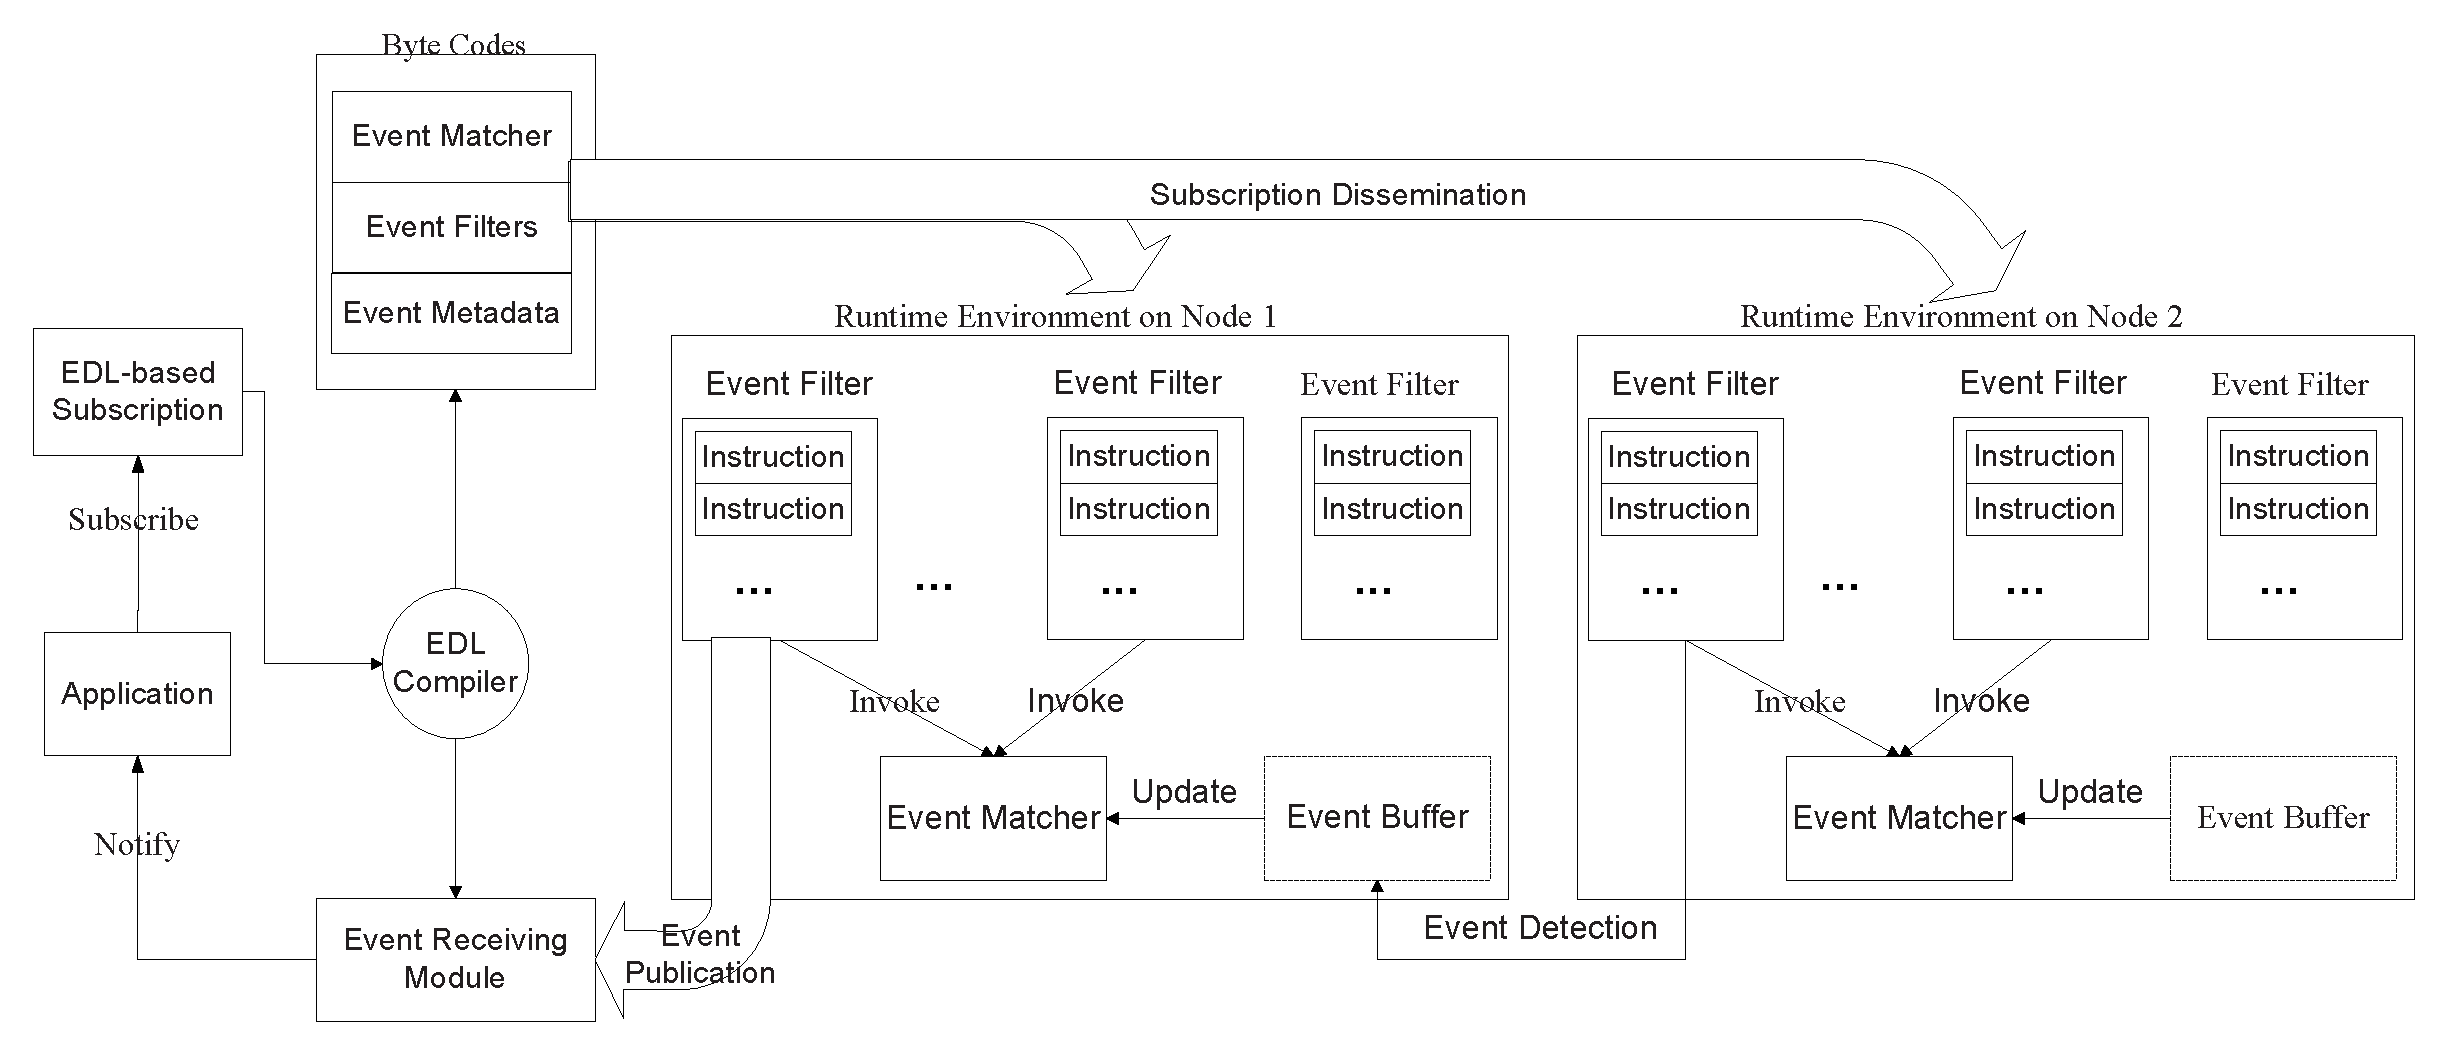
\includegraphics[width=\textwidth]{psware-interaction-simple}
\caption{PSWare-E components interaction}
\label{fig:psware-interaction-simple}
\end{figure*}

\subsection{EDL and Its Compiler}
The subscription contains one or more event definition and one subscribing statement. Formally, the BNF of the subscription is defined in Listing \ref{prog:BNFSubscription}.

\begin{lstlisting}[caption=BNF (simplified) of subscription, label=prog:BNFSubscription]
subscription -> event_declarations subscribe_statement
event_declarations -> event_declaration | event_declarations event_declaration
subscribe_statement -> SUBSCRIBE IDENTIFIER SEMICOLON
\end{lstlisting}

The subscribe statement simply uses the keyword 'subscribe' followed the event type name needed by the application. Each event type declaration can have up to three parts: the event body, the where clause and the on clause. The event body defines the attributes of the events. The on clause are used to specify the sub-events used by a composite event. The where clause defines the filter of the corresponding event type. Formally, the BNF of event type is defined in Listing \ref{prog:BNFEvent}

\begin{lstlisting}[caption=BNF (simplified) of event type, label=prog:BNFEvent]
event_declaration -> EVENT IDENTIFIER event_body on_clause_opt where_clause_opt
event_body -> { field_declarations_opt }
on_clause -> ON { subevent_declarations_opt }
where_clause -> WHERE { conditional_expression }
\end{lstlisting}

The on clause and the where clause are both optional in case if the event is primitive or doesn't have a filter. The on clause looks similar to the field declaration except sub-events instead of fields are declared. This is done for a clear code presentation and easier type checking. The where clause simply consists of conditional expressions so that the filters may be defined by specifying the operators.

A simple example of using EDL is shown in Listing \ref{prog:originaledl}. In this example, two events, 'SimpleEvent' and 'CompEvent' are defined. 'SimpleEvent' is a primitive event which occurs when the detected temperature reading is above certain threshold. 'CompEvent' is a composite event that is based on two events of 'SimpleEvent' and their time must satisfy a certain condition in order to indicate the occurrence of 'CompEvent'.
\begin{lstlisting}[caption=A simple EDL program, label=prog:originaledl]
Event SimpleEvent {
	int temp=System.temp;
	int id=System.id;
	int time=System.time;
} where {
	temp > 30
}
Event CompEvent {
} on {
	SimpleEvent e1 and
	SimpleEvent e2
} where {
	e2.time-e1.time=600
}
\end{lstlisting}

The EDL-based subscription will be processed by our EDL compiler. The output of the compiler has two parts as shown in Figure \ref{fig:edlcompiler}. The first part is the byte codes which will be executed by individual sensors to detect events. We will discuss how the sensor nodes will execute the byte codes in the next section. The second part is the event receiving module. This module is responsible for receiving and interpreting the events delivered from WSN and notify the application layer if the subscribed events are delivered.

\begin{figure}
\centering
\figurecurrentwidth{edlcompiler}
\caption{EDL compiler structure}
\label{fig:edlcompiler}
\end{figure}

\subsection{Event Detection Framework}
The byte codes generated by the compiler can be further divided into three parts: event meta data, event filters and event matcher. Event meta data contains the description of the event types such as event type ID, event size and the individual attributes for each event. Event filters are the constraints defined for each event type. Event matcher schedules the execution for event detection according to the subscription and event relations.

The runtime environment on each sensor node is similar to the VM-based approach \cite{mate} in the sense that the subscriptions are broken down into some basic operations. Such design choice is for the extensibility of the middleware so that different event detection mechanisms may be easily implemented through the operations. In addition to the VM-based runtime environment, as shown in Figure \ref{fig:pswarevm}, each sensor node has an event buffer where the detected events may be stored for composite event detection.

\begin{figure}
\centering
\figurecurrentwidth{pswarevm}
\caption{PSWare runtime environment}
\label{fig:pswarevm}
\end{figure}

The essential operations for our event detection framework is shown in Figure \ref{fig:eventdetectionframework2}. In this framework, the event matcher will first fetch the events from the event buffer and then evaluate them against the corresponding filters. If the event has been detected, then it will be transmitted over the network. Formally, the procedure of the event matcher can be shown in Procedure \ref{algo:eventmatcher} with some notations defined as:
\begin{itemize}
\item Event types: \(E=\{e_1, e_2 \cdots \}\)
\item For each \(e_n\in E\), its filter is: \(e_n\rightarrow filter\)
\item For each \(e_n\in E\), it has a set of events \(E_n=\{e_n^1, e_n^2 \cdots \}\) stored in the buffer.
\end{itemize}

\begin{figure}
\centering
\figurecurrentwidth{eventdetectionframework2}
\caption{Event detection framework}
\label{fig:eventdetectionframework2}
\end{figure}

\begin{algorithm}
\begin{algorithmic}
\REQUIRE \(E\)
	\FORALL {\(e_n\in E\)}
		\FORALL {\(e_n^i\in E_n\)}
			\IF {\(e_n\) is primitive}
				\STATE result = evaluate\_primitive (\(e_n^i\))
				\IF {result == True}
					\IF {\(e_n\) is subscribed}
						\STATE deliver(\(e_n^i\))
					\ELSE
						\STATE forward(\(e_n^i\))
					\ENDIF
				\ENDIF
			\ELSE
				\FORALL {subevents \(e_m\) for \(e_n\)}
					\STATE evaluate\_composite(\(e_n^i\), \(e_m\), \(\cdots \))
				\ENDFOR
			\ENDIF
		\ENDFOR
	\ENDFOR
\end{algorithmic}
\caption{Procedure of the event matcher}
\label{algo:eventmatcher}
\end{algorithm}

There are several keys in the procedure. First, when the event matcher picks up the events of type \(e_n\) from the event buffer, it may use application specific mechanisms to pick up the desired events instead of trying all the possible combinations. Second, the 'deliver()' and the 'forward()' function are used to deliver the subscribed events or forward the events so that composite events may be detected. These two functions may also be application dependent to achieve high energy efficiency.

Figure \ref{fig:psware-interaction-simple} illustrates how different components in the middleware system interact with each other.

\subsection{Customizing PSWare}
The event detection framework of PSWare is developed using NesC. As discussed in the previous section, many of the operations in PSWare can be defined according to applications. In this section, we describe how we can customize PSWare.

The first step is to implement a special module which acts like a device driver for PSWare. This module defines the sampling rate and a primitive event called 'System'. All the fields of other events are obtained from 'System'. The module needs to implement three interfaces: StdControl, SystemClock and SystemEvent as shown in Listing \ref{prog:systemEvent}. StdControl is a module for initialization purpose. SystemClock defines the sampling frequency. SystemEvent is used to obtain the pointer to the 'System' event.

\begin{lstlisting}[caption=API of the 'System' event, label=prog:systemEvent]
module SystemEventM {
	provides {
		interface StdControl;
		interface SystemEvent;
		interface SystemClock;
	}
}
interface SystemEvent {
	command EventInstanceInfo * get();
}
\end{lstlisting}

Once the 'System' event is defined, the application developers can further define their own functions for event delivery and event forwarding. We will show some examples in the next section. In addition, they can make use of the API provided by PSWare as shown in Listing \ref{prog:pswareAPI}.

\begin{lstlisting}[caption=API provided by PSWare, label=prog:pswareAPI]
interface EventMeta {
	command EventMetaInfo * getEventMeta(uint8_t subID);
	command bool isSubscribed(uint8_t subID);
	command bool isComposite(uint8_t subID);
	command bool isAggregate(uint8_t subID);
}
interface EventInstance {
	command EventInstanceInfo * createEvent(uint8_t subID);
	command int instanceAmount(uint8_t subID);
	command void deleteEvent(uint8_t subID, uint8_t instanceID);
	command EventInstanceInfo * getEventInstance(uint8_t subID, int idx);
}
interface EventMatcher {
	command bool selectSubevent(EventInstanceInfo * composite, EventInstanceInfo * subevent);
	command result_t eventDetected(uint8_t subID, uint8_t instanceID, bool detectionResult);
	command result_t eventDelivery(uint8_t subID, uint8_t instanceID, bool detectionResult);
}
\end{lstlisting}

These API provides the necessary functionalities for accessing modules such as event meta data or the event buffer (as in EventInstance). To implement application specific event detection mechanisms, application developers simply need to override the commands provided in the EventMatcher interface. The 'selectSubevent()' command is used to determine if a sub-event (in the parameter subevent) should be used to detect a composite event (in the parameter composite).